\documentclass[11pt]{article}

\usepackage[margin=1in]{geometry}
\usepackage{graphicx}
\usepackage{booktabs}
\usepackage{hyperref}
\usepackage{amsmath}
\usepackage{float}
\usepackage{siunitx}

\title{COMS E6424 Hardware Security\\Homework 3 Reflection Report}
\author{Peiheng Li(pl2978)~~~~~Peng Chen(pc3193)\\Wenxuan Xu(wx2341)~~~~~Xiangyu Liao(xl3581)~~~~~Yinfeng Chai(yc4669)}
\date{\today}

\begin{document}
\maketitle

\section{Overview}
This homework asked us to build a covert channel between two user processes running on the same VM without using an overt communication path. Our implementation still uses the same physical idea as before: a Flush+Reload channel built around the shared \texttt{libc} symbol \texttt{ecvt\_r}. A cache-hot slot carries a \texttt{1}. A flushed slot carries a \texttt{0}. The receiver probes the same function, times it with \texttt{RDTSCP}, and converts the resulting timing pattern into bits.

The main change in the final version is above the physical layer. Instead of repeating one ad hoc frame forever, we now send a packet stream. A long message is split into fixed-size payload chunks, each chunk is wrapped in a small header, and the receiver reassembles the original text from validated packets. In practice, this changed the system from ``a covert channel that can print one short string'' into ``a covert channel that can transport a longer text as a sequence of datagrams.'' That was the real goal.

\section{Techniques We Tried and Why}
Our starting point was the appendix code. It was useful for verifying the basic microarchitectural effect, but it was not a complete transport mechanism. The earliest version simply measured one call to \texttt{ecvt\_r}, compared the timing against a threshold, and emitted raw bits. That was enough to show that the cache state was observable. It was not enough to move a message in a controlled way.

The first improvement was slotting. Both processes divide time into fixed windows using \texttt{CLOCK\_MONOTONIC}. Once the bit duration is known on both sides, they implicitly agree on bit boundaries. The sender uses the current slot number to decide which bit to place on the channel, and the receiver spends the whole slot probing and deciding whether the slot looked mostly hot or mostly cold. This was much more stable than treating each bit as a single timing sample.

The second improvement was framing, and later packetization. The intermediate version added a sync word and a payload length, which already made the channel easier to align. The current version goes one step further and uses a small one-way packet protocol. Each packet carries a version-and-flags byte, a session identifier, a packet index, the total packet count, a payload length, the payload itself, and a CRC-16. The sender repeats the packet train indefinitely, so the receiver can start in the middle of a transmission and still collect missing packets over later cycles. Since the receiver cannot acknowledge anything, this kind of one-way redundancy is much more useful than a stop-and-wait design.

We also tested immediate packet duplication inside the same transmission cycle. The idea was straightforward: if one copy is damaged, the second may survive. In four quick \SI{1}{ms} trials with a 61-byte message, however, both \texttt{-r 1} and \texttt{-r 2} completed 4/4 times on our machine, while the average completion time increased from about \SI{1.02}{s} to \SI{1.30}{s} with \texttt{-r 2}. Because the full packet train is already retransmitted forever, we kept \texttt{-r} as an option for noisier setups but set the default to \texttt{1}.

\section{Implementation Summary}
The submission now consists of three C programs and one shared header.

\texttt{threshold.c} is still the calibration tool. It measures \texttt{ecvt\_r} after flushed and non-flushed conditions and reports the timing statistics needed to choose a threshold.

\texttt{sender.c} now packetizes the input message. By default it uses 16 payload bytes per packet. It supports both \texttt{-m} for a command-line string and \texttt{-f} for reading a longer text from a file. Each packet is serialized as
\[
  [\texttt{A5 5A}][\texttt{version+flags}][\texttt{session\_id}][\texttt{packet\_index}][\texttt{packet\_count}][\texttt{payload\_len}][\texttt{payload}][\texttt{crc16}].
\]
\[
\begin{array}{l|c|c|c|c|c|c|c}
\textbf{Field} & \texttt{SYNC} & \texttt{V{+}FLG} & \texttt{SESSION} & \texttt{PACKET\_IDX} & \texttt{PACKET\_CNT} & \texttt{PL\_LEN} & \texttt{PAYLOAD} \;|\; \texttt{CRC16} \\
\hline
\textbf{Length} & 2\text{ B} & 1\text{ B} & 2\text{ B} & 2\text{ B} & 2\text{ B} & 1\text{ B} & 0\text{--}64\text{ B} \;|\; 2\text{ B}
\end{array}
\]

The sender then transmits the resulting byte stream one bit per time slot.

\texttt{receiver.c} probes the channel one slot at a time, searches for the sync word, parses packets, checks the CRC, stores valid packets by sequence number, and prints the reconstructed message once all packets for the current session have been received. Importantly, an ambiguous bit no longer destroys the whole reassembly state. It only causes the receiver to drop the current partial packet and look for the next sync word.

\texttt{protocol.h} holds the shared wire-format constants, little-endian helpers, and the CRC-16 implementation. Keeping those definitions in one place made it much easier to keep sender and receiver consistent while the protocol was changing.

\section{Threshold Tuning}
On our test machine the threshold tuner consistently produced two clusters. A short calibration log is included with the submission in \texttt{report\_assets/threshold\_measurements.txt}, and the raw samples behind the paper-style distribution in Figure~\ref{fig:threshold-dist} are saved in \texttt{report\_assets/threshold\_distribution.csv}. In the later portion of the tuner log, the non-flushed average settles around \SI{360}{cycles} to \SI{370}{cycles}, while the flushed average settles around \SI{815}{cycles} to \SI{820}{cycles}. We therefore used \SI{600}{cycles} as the receiver threshold. That choice is conservative, but it sits in the gap between the two groups and worked well in our tests.

\begin{figure}[H]
    \centering
    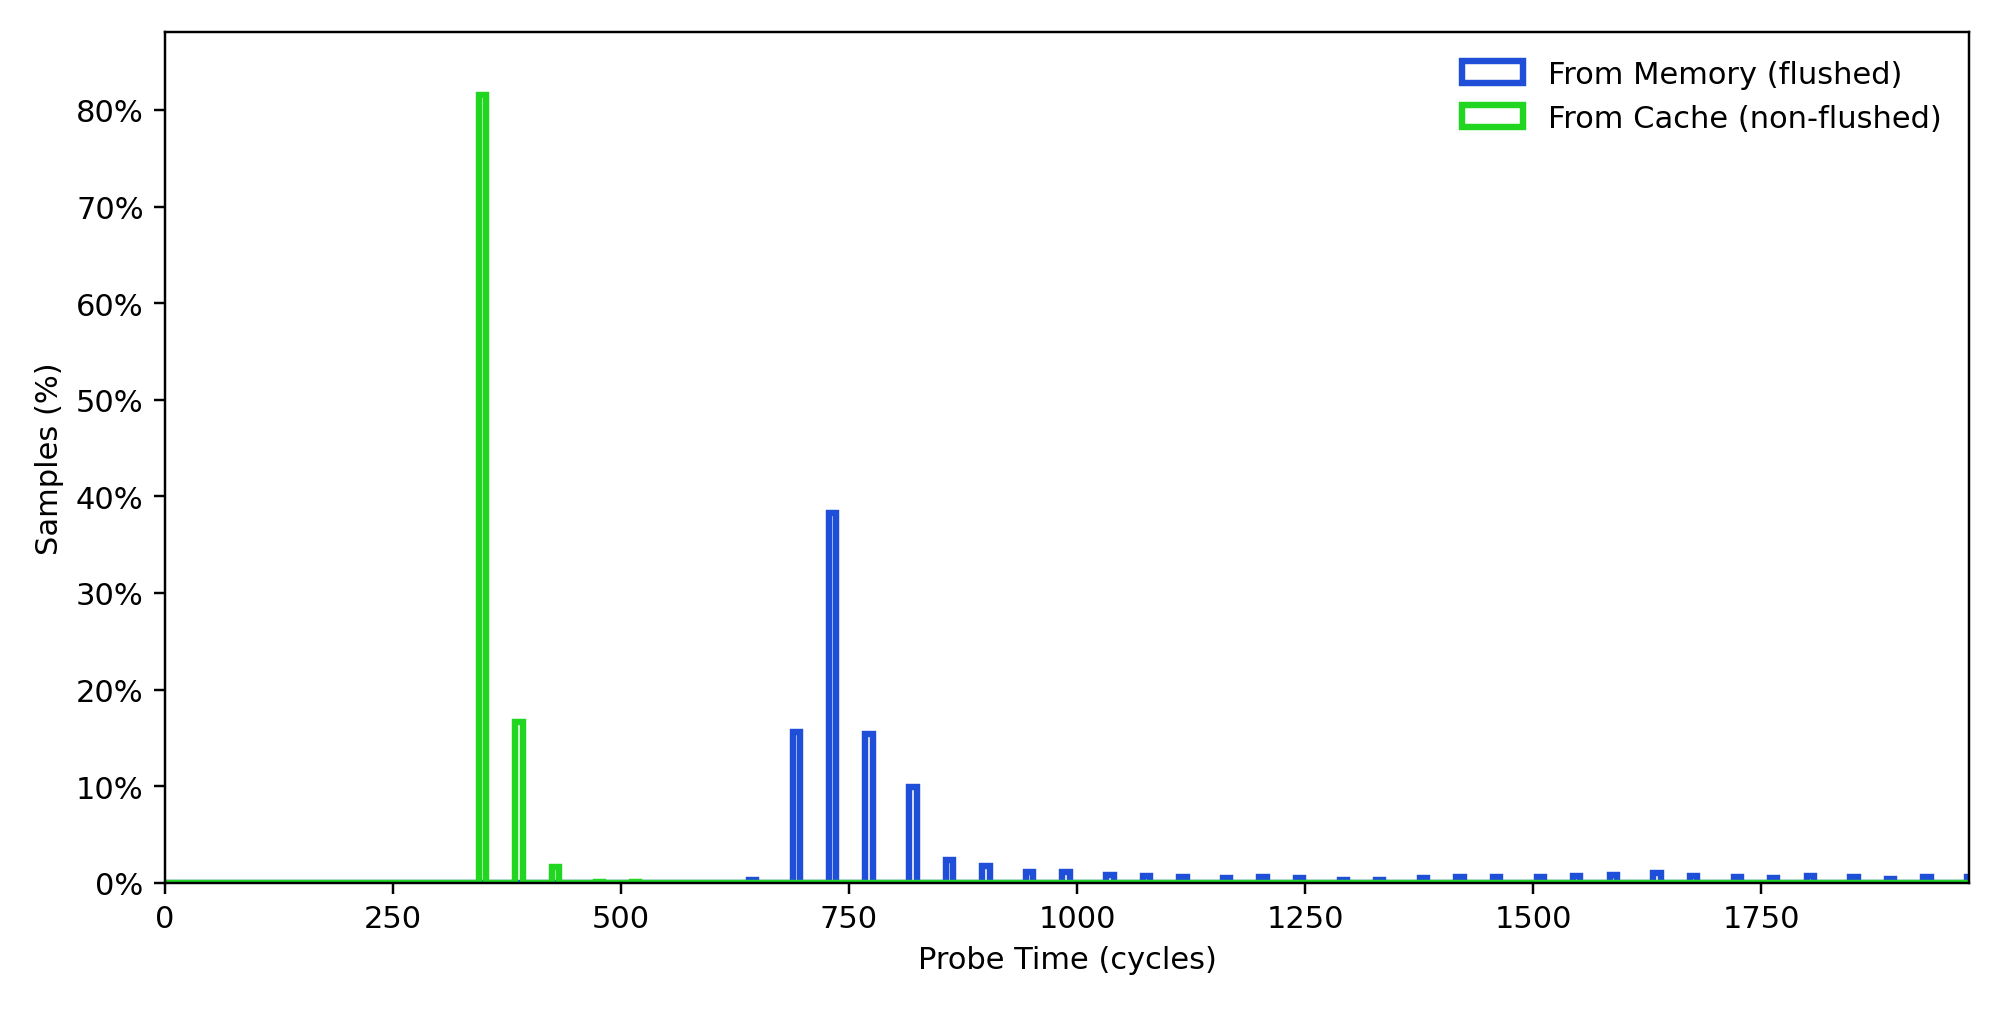
\includegraphics[width=0.94\linewidth]{report_assets/threshold_distribution.png}
    \caption{Distribution of isolated \texttt{ecvt\_r} probe times collected with the same flush/non-flush experiment as \texttt{threshold.c}. The plot is intentionally styled after the load-time distribution figure in the original Flush+Reload paper, but it is generated from our own measurements. We collected 5000 flushed samples and 5000 non-flushed samples. The non-flushed accesses cluster near \SI{350}{cycles}, while the flushed accesses peak near \SI{730}{cycles} and show a longer tail.}
    \label{fig:threshold-dist}
\end{figure}

The threshold is still machine-dependent. Nothing in the higher-level packet protocol relies on \SI{600}{cycles} specifically; only the physical-layer classifier does. On another VM, the correct threshold may move, but the packet format and reassembly logic can remain unchanged.

These calibration numbers are not supposed to match the plot in Figure~\ref{fig:probe-trace}. Figure~\ref{fig:threshold-dist} shows isolated single-call timings. Figure~\ref{fig:probe-trace} shows slot-level average probe times while the packetized sender is actively running. During a \texttt{0} bit, the sender keeps flushing the target throughout the slot, so the observed average becomes much larger than the single-flush calibration number.

\begin{figure}[H]
    \centering
    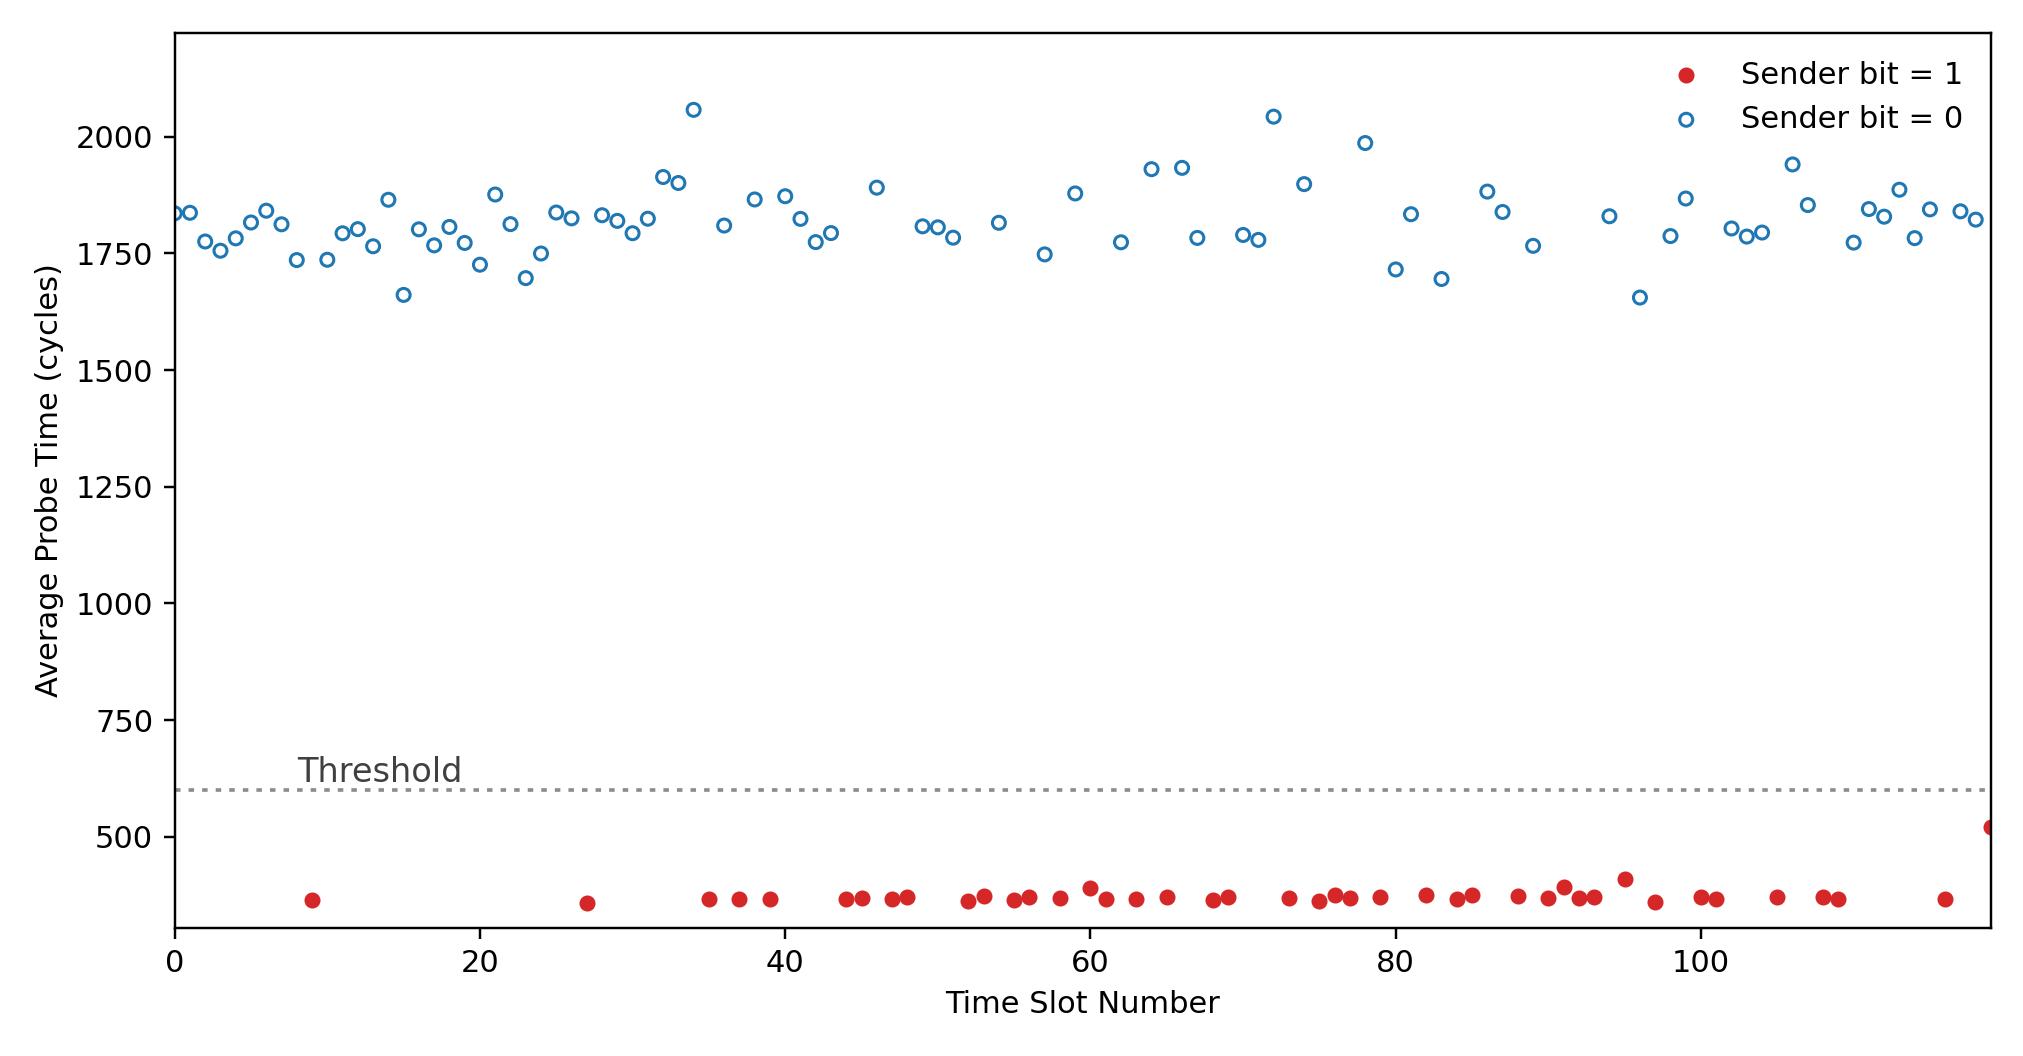
\includegraphics[width=0.92\linewidth]{report_assets/probe_trace.png}
    \caption{Probe-time measurements for \texttt{ecvt\_r} over 120 consecutive time slots while the sender transmits a 61-byte packetized message at \SI{5}{ms} per bit. The figure follows the style of the probe-time plot in the original Flush+Reload paper, but it is generated from our own implementation and our own measurements. On this run the hot cluster stays near \SI{375}{cycles}, while the flushed cluster rises to roughly \SI{1.8e3}{cycles}.}
    \label{fig:probe-trace}
\end{figure}

Figure~\ref{fig:probe-trace} shows why the channel works. Even on a virtualized machine, the two groups are still clearly separated. The packet protocol only helps if the physical bit classifier is clean enough to supply useful bits in the first place.

\section{Expected Bandwidth Versus Measured Bandwidth}
For the packetized measurements below, we used the message \texttt{Packetized covert channels survive duplicates and CRC checks.}, which is 61 bytes long. With a 16-byte payload size, that message becomes four packets. One full transmission cycle contains 109 bytes on the wire, or 872 transmitted bits. Since the message itself carries 488 payload bits, the ideal cycle-limited payload goodput is
\[
R_{\text{ideal}} = \frac{488}{872d},
\]
where \(d\) is the bit duration in seconds.

To measure the updated protocol, we started the receiver, launched the sender, and timed how long it took until the first fully reassembled message appeared. Table~\ref{tab:bandwidth} reports both the ideal cycle-limited goodput and the observed completion rate, where the completion rate is just payload bits divided by the measured completion time.

\begin{table}[H]
    \centering
    \sisetup{round-mode=places,round-precision=1}
    \setlength{\tabcolsep}{4pt}
    \renewcommand{\arraystretch}{1.08}
    \resizebox{\linewidth}{!}{%
    \begin{tabular}{@{}rrrrl@{}}
        \toprule
        Bit dur. (ms) & Ideal goodput (bps) & Completion time (s) & Completion rate (bps) & Notes \\
        \midrule
        10 & 56.0 & 9.19 & 53.1 & Stable \\
        5  & 111.9 & 4.66 & 104.8 & Stable \\
        2  & 279.8 & 2.11 & 230.9 & Works well \\
        1  & 559.6 & 1.69 & 288.8 & Higher variance \\
        \bottomrule
    \end{tabular}%
    }
    \caption{Measured behavior of the packetized protocol for a 61-byte message split into four packets with 16 payload bytes each. The completion rate is based on time to first fully reassembled message.}
    \label{tab:bandwidth}
\end{table}

\begin{figure}[H]
    \centering
    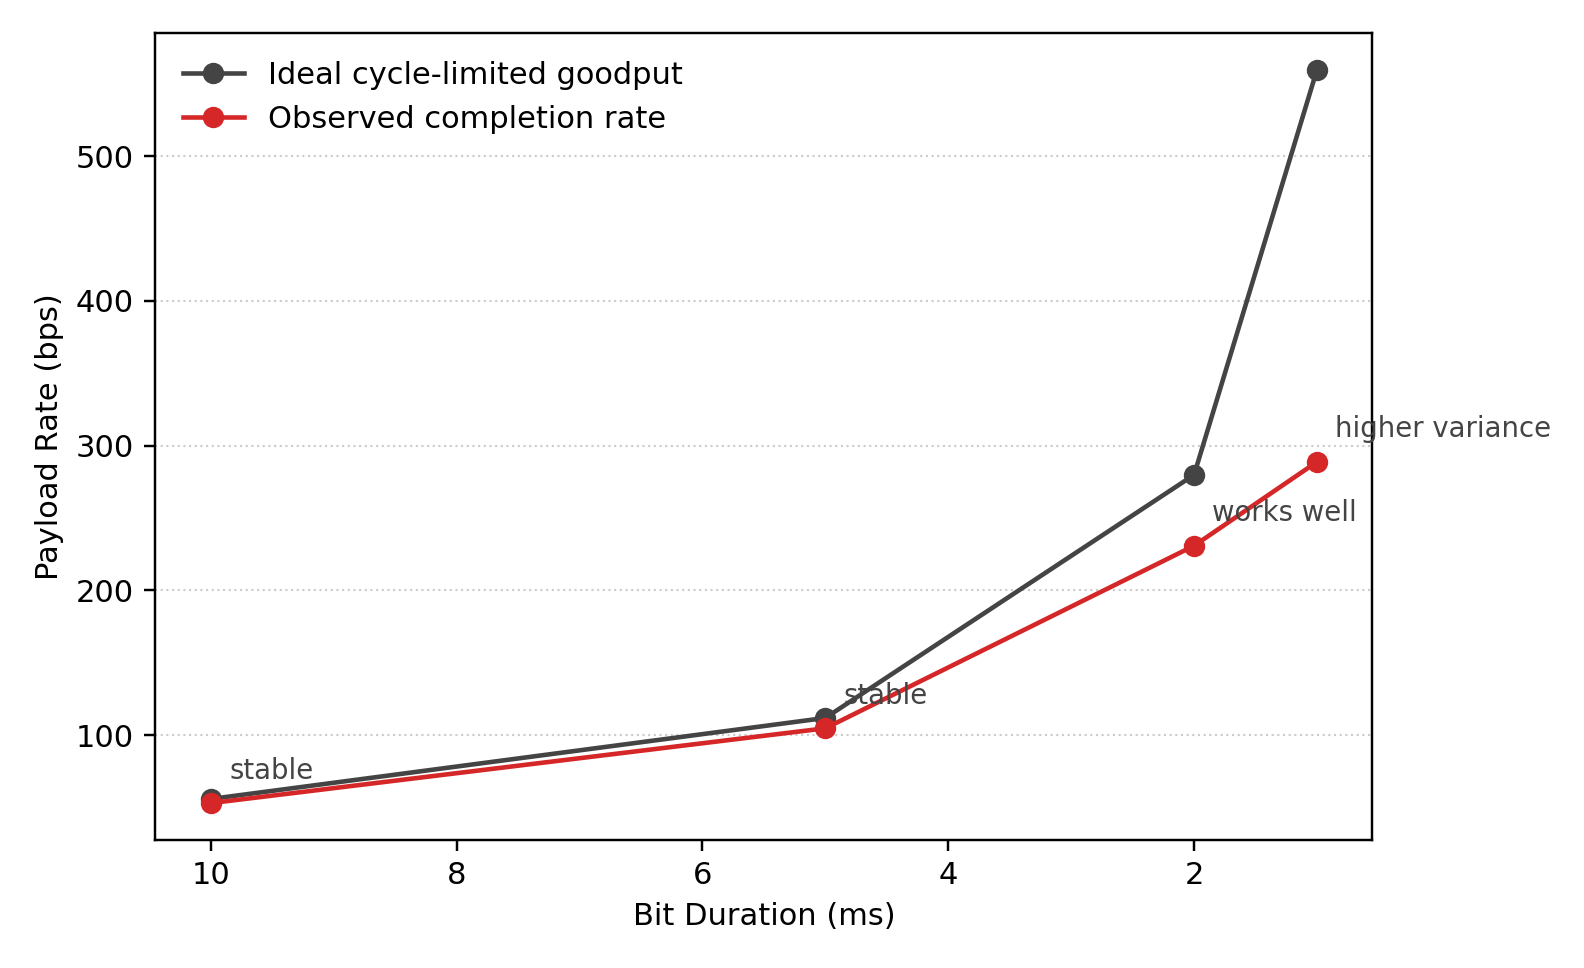
\includegraphics[width=0.82\linewidth]{report_assets/bandwidth_sweep.png}
    \caption{Ideal cycle-limited payload goodput versus observed completion rate for the packetized protocol. The two curves remain close at \SI{10}{ms} and \SI{5}{ms}. At \SI{2}{ms} and especially \SI{1}{ms}, the message still arrives, but the receiver spends more time waiting for the missing packets that complete the set.}
    \label{fig:bandwidth}
\end{figure}

The behavior is different from the earlier single-frame version, and that is expected. Once the message is packetized, the receiver no longer needs one perfectly decoded frame. It only needs one valid copy of each packet. This improves robustness, especially when the receiver starts in the middle of a transmission. At the same time, there is more protocol overhead: headers, CRC, and packet boundaries all cost bits. That is the tradeoff.

On our machine, \SI{5}{ms} is a comfortable setting. It delivered the full 61-byte message in about \SI{4.66}{s}, which corresponds to roughly \SI{105}{bps} of useful payload. \SI{2}{ms} still worked well and brought the completion time down to about \SI{2.11}{s}. At \SI{1}{ms}, the protocol still completed in our tests, but the timing was clearly less stable. This is exactly the kind of behavior the packet design was meant to improve: instead of failing catastrophically, the receiver can wait for whichever packet did not arrive cleanly on the first pass.

We also tested the file-input path with an 84-byte text file stored as \texttt{report\_assets/test\_payload.txt}. At \SI{2}{ms}, the receiver reconstructed the full six-packet message and printed the original text correctly. That test was important because a packet protocol is much more useful when it can accept a longer input than what is practical to type directly on the command line.

\section{Hardware and Reproducibility}
Our measurements were taken on a Linux guest running under WSL2 on an AMD Ryzen 9 9950X3D system. The guest reports 32 logical CPUs, \texttt{clflush}, and \texttt{rdtscp} support. The environment still matters. This is a VM, so there is scheduler noise and hypervisor interference, but the shared-library code pages are available to both processes, which is exactly what Flush+Reload needs.

To reproduce the current packetized experiment:

\begin{enumerate}
    \item Compile with \texttt{make}.
    \item Run \texttt{./threshold} and choose a threshold between the flushed and non-flushed timing clusters. On our machine, \SI{600}{cycles} worked well.
    \item Start the receiver, for example \texttt{./receiver -t 600 -d 5}.
    \item Start the sender, for example \texttt{./sender -m "Packetized covert channels survive duplicates and CRC checks." -d 5 -p 16}.
    \item For longer text, use \texttt{-f} instead of \texttt{-m}. For noisier settings, \texttt{-r 2} remains available as an optional redundancy knob.
\end{enumerate}

\section{Reflection}
The most useful lesson from this homework was that the microarchitectural channel itself is only part of the system. A good transport layer matters just as much. Without it, the receiver sees a stream of timings and hopes they line up. With it, the receiver has structure: packet boundaries, packet numbers, a way to reject corruption, and a clear rule for when the message is complete.

That changed the failure mode in a good way. The older design could lose the message if one portion of the frame went bad. The packetized design is more forgiving. If one packet is damaged, the receiver drops that packet, keeps the valid ones it already has, and waits for the missing piece to reappear in a later cycle. That is a much more realistic behavior for a one-way channel.

If we had more time, the next step would probably be a stronger forward-error-correcting code inside each packet, or a checksum over the whole reassembled message in addition to the per-packet CRC. We would also look at CPU pinning and perhaps a smaller probe window jitter margin on quieter machines. The current protocol is already much more useful than the original frame-only design, but it still leaves room for tuning.

\section{Conclusion}
We implemented a working packetized covert channel on top of the Flush+Reload physical layer. The sender now breaks long text into numbered packets, the receiver validates those packets with CRC-16, stores them by sequence number, and reconstructs the original message once all packets have arrived. On our test platform, this design carried multi-packet messages reliably at \SI{5}{ms} and remained usable down to \SI{1}{ms}, with the expected increase in timing variance at the fastest setting.

\begin{thebibliography}{9}
\bibitem{yarom2014}
Yuval Yarom and Katrina Falkner,
\textit{Flush+Reload: A High Resolution, Low Noise, L3 Cache Side-Channel Attack},
USENIX Security Symposium, 2014.

\bibitem{hw3}
COMS E6424 Hardware Security Homework \#3, Spring 2026.
\end{thebibliography}

\end{document}
